\documentclass[runningheads,a4paper,fleqn]{llncs}

\usepackage{amsmath}
\usepackage{amssymb}
\usepackage{alltt}
\usepackage{lineno}
\usepackage{graphicx}
\usepackage[normalem]{ulem}


\begin{document}

\title{Multi-Lane FlowPools: A detailed look}
\author{Tobias Schlatter}

\institute{EPFL, Switzerland}

%% TODO how to add advisor, etc.

\maketitle

\begin{abstract}
  FlowPools, proposed by \cite{FP12} are a powerful way to express
  dataflow logic in highly parallelized applications. The original
  paper proposes two ways of implementing a FlowPool: Single-Lane
  FlowPools (SLFP) and Multi-Lane FlowPools (MLFP). While SLFPs are
  relatively simple to implement, insertions do not scale. MLFPs solve
  this limitation. This report goes into the details of the
  implementation of MLFPs and analyzes some benchmarking results in
  more detail to show that insertions MLFPs scale nicely, with respect
  to SLFPs, and other concurrent data structures.
\end{abstract}

\section{Introduction}
The goal of this section is to briefly remind the reader of the
semantics and programming interface of a FlowPool and the basic ideas
behind the implementation of SLFPs to allow for better understanding
of the implementation of MLFPs.

\subsection{Programming Model}
The following operations are supported by a FlowPool. For a proof of
determinism, refer to \cite{FP12}.

\textbf{Append (\texttt{<<})} Inserts an element in the
FlowPool. Fails if the number of elements the FlowPool has been sealed
with is reached.\\
Signature: \verb+def <<(x: T): Unit+

\textbf{Foreach} Traverse elements in the FlowPool. Calls a closure
\verb+f+ exactly once (asynchronously) for each element added to the
FlowPool (until it is sealed). Returns future of number of elements in
pool.\\
Signature: \verb+def foreach[U](f: T => U):+ \verb+Future[Int]+

\textbf{Aggregate} Reduce elements in the FlowPool to a single
value. Starts off with \verb+zero+ as initial value to aggregate on,
calls \verb+op+ exactly once per element to add it to an aggregation,
finally uses \verb+cb+ to combine multiple aggregations into a single
one. Note that \verb+op+ is guaranteed to be executed only once per
element, whereas \verb+cb+ may be called any number of times\\
Signature: \verb+def aggregate[S]+\verb+(zero: =>S)+
\verb+(cb: (S, S) => S)+\\
\verb+(op: (S, T) => S):+ \verb+Future[S]+

\textbf{Builders} Abstraction to allow garbage collection of elements
that are no longer required. Allows insertion without reference to
initial pool (and hence all elements). See \cite{FP12} for details.

\textbf{Seal} Fixes the number of elements that will eventually be in
the pool allowing callbacks to be freed once reached. The final size
of the pool is required as argument in order to preserve the
determinism of the model. Subsequent call to \verb+seal+ will fail iff
the FlowPool has already been sealed with a different size or the
number of elements in the FlowPool is larger than the seal size.\\
Signature: \verb+def seal(size: Int): Unit+

\subsection{Single-Lane FlowPool}
SLFPs are implemented using a single linked-list of arrays of
elements, where the last non-empty element does not hold actual data,
but the state of the FlowPool, i.e. a list with all the callbacks and
the seal state of the FlowPool. Changes to the SLFP are only allowed
by CASing at this particular point, which hence serves as
linearization point of the datastructure.

With competing, concurrent writers, this approach does not scale
nicely (see figure~\ref{fig:eval-cpu-scaling}). Mainly due to cache
contention (multiple CPUs often write to close memory locations) and
CAS collisions.

\section{Implementation}
MLFPs take advantage of the lack of ordering guarantees in the
FlowPool semantics to remove the limitation of SLFPs with respect to
scaling by applying a simple but effective idea: Instead of having a
single SLFP, we use one SLFP for each processor (or thread). This
means, that on one hand, every processor (or thread) gets its own list
of arrays to which he appends elements to, avoiding CAS collisions and
cache contetion. On the other hand, every callback or aggregation has
to be registered on each of these lanes seperately.

\subsection{Seal}

\subsection{Callbacks}



\subsection{Insertion}

\section{Evaluation}

\begin{figure}
\centering
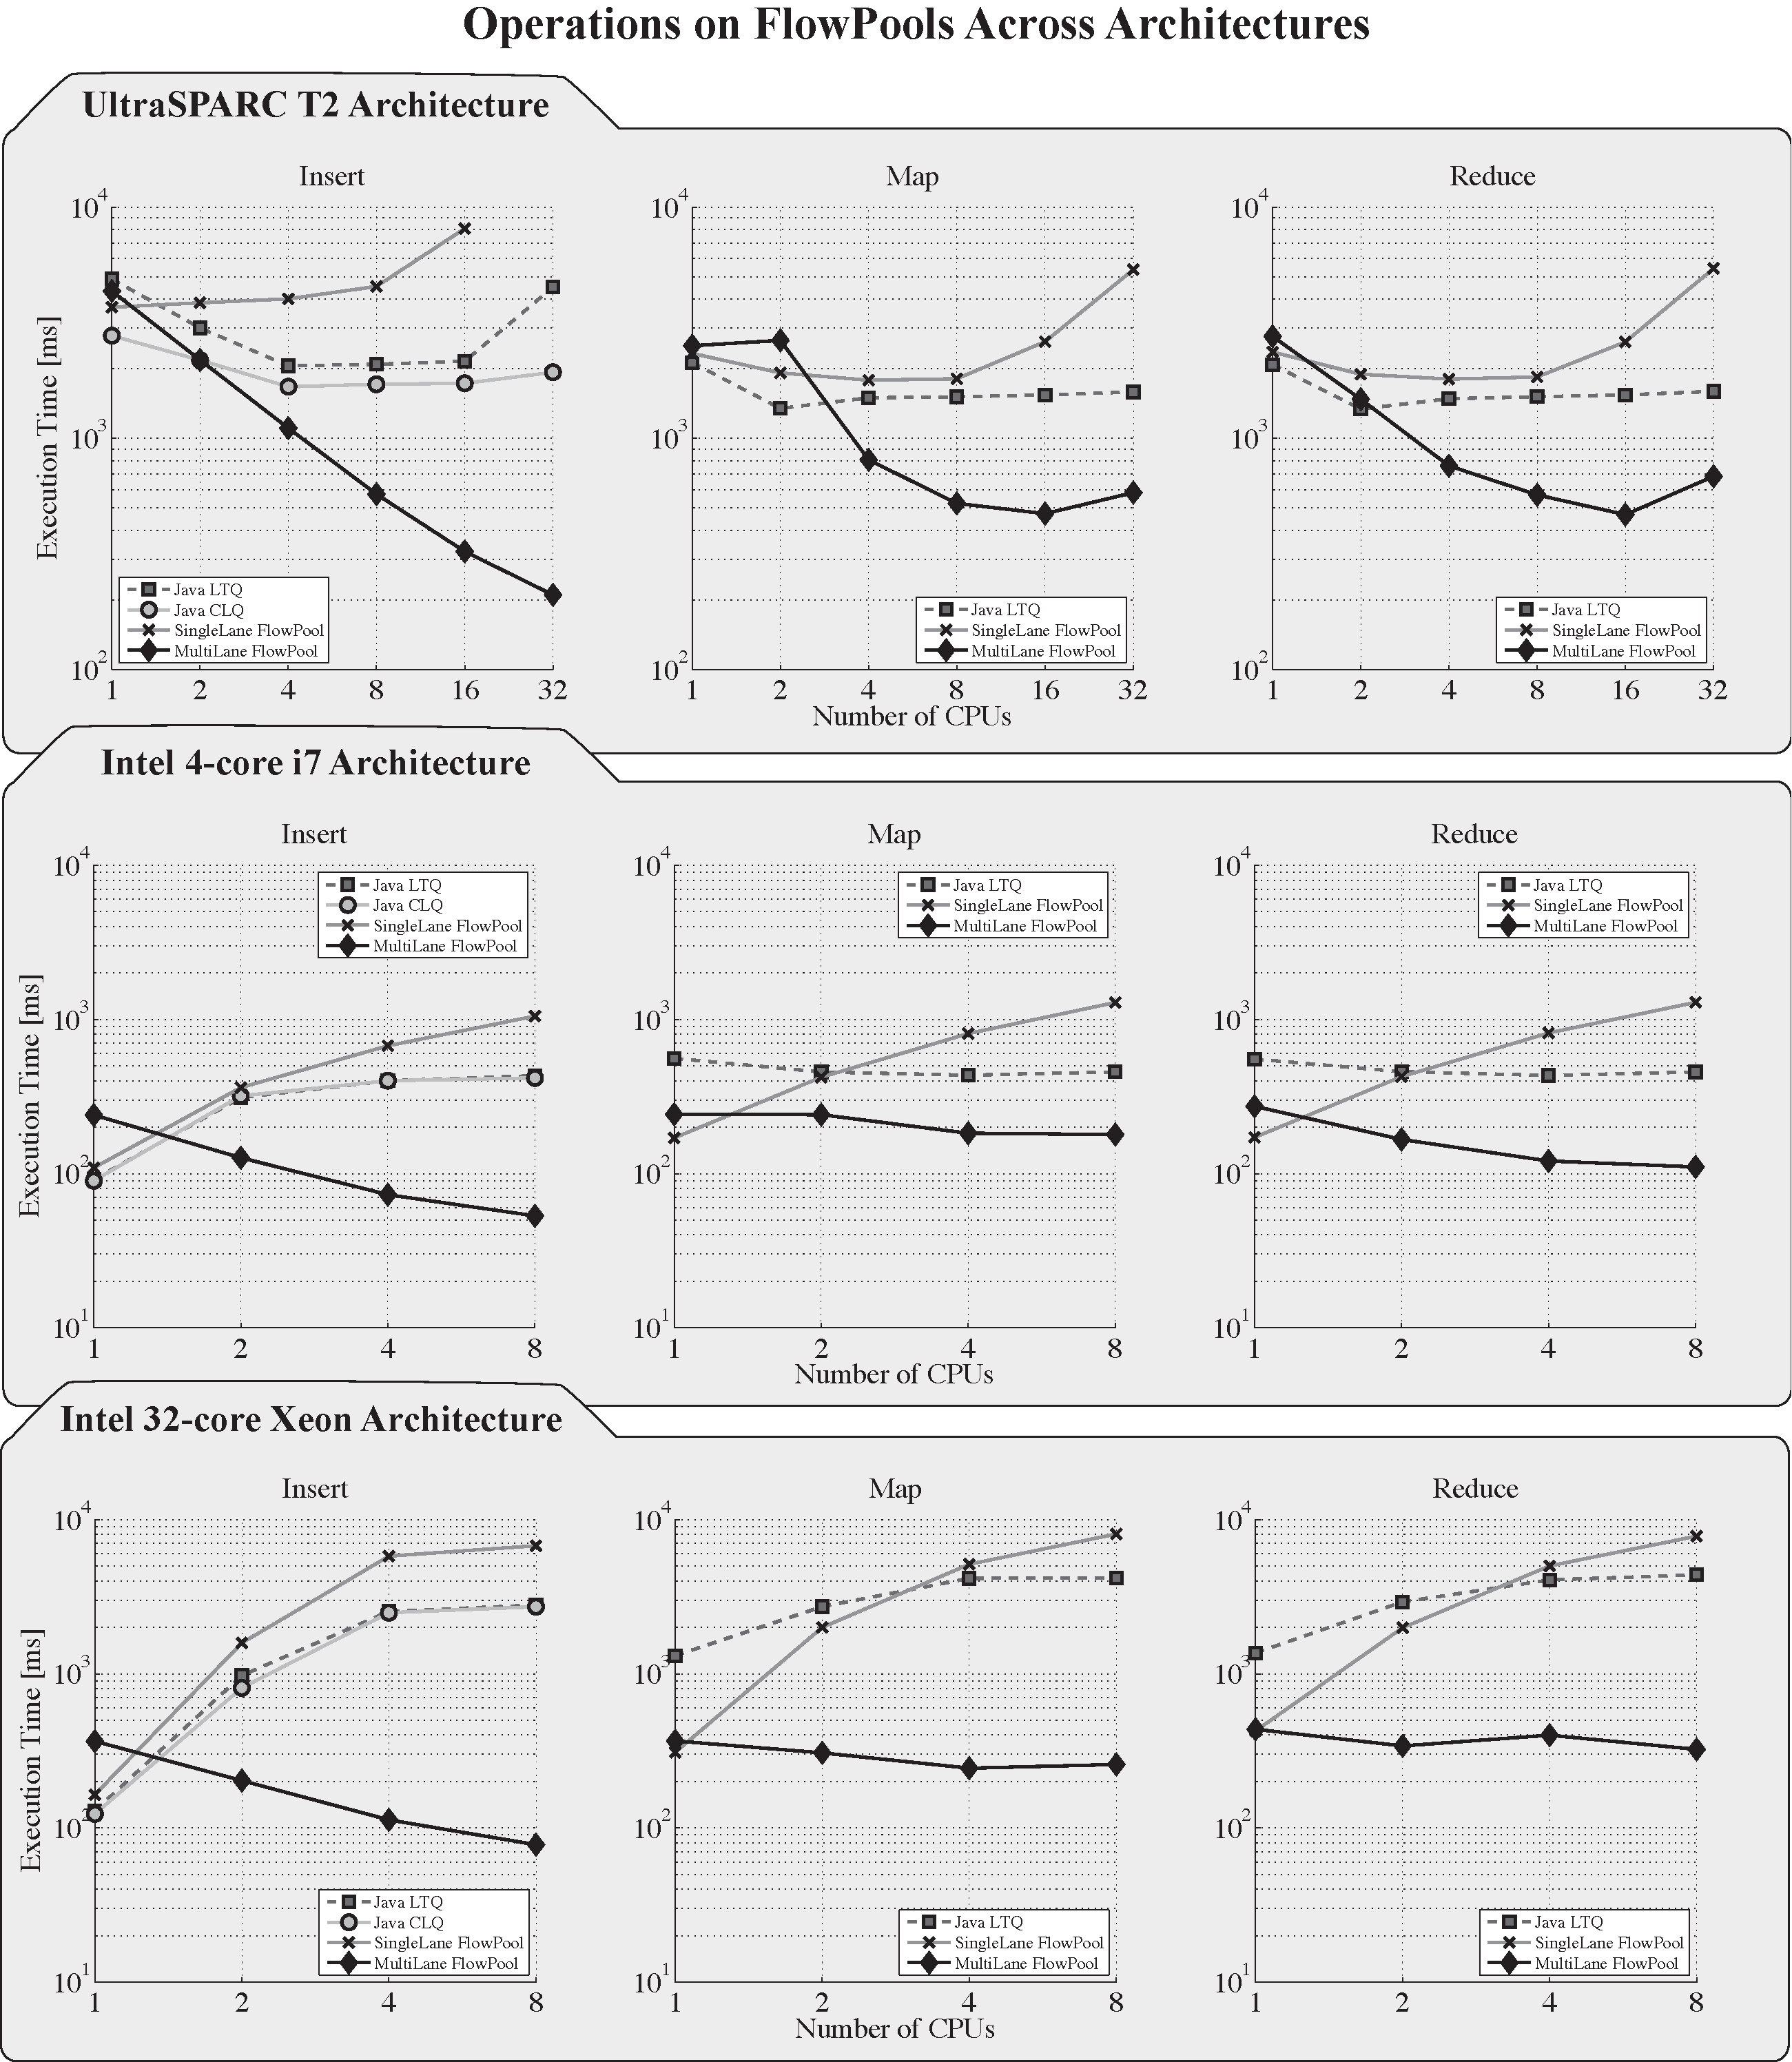
\includegraphics[width=\textwidth]{../../benchmarks/graphs/scaling-operations}
\setlength{\abovecaptionskip}{-10pt}
\setlength{\belowcaptionskip}{-20pt}
\caption{Execution time vs parallelization across three different
architectures on three important FlowPool operations; insert, map, 
reduce.}
\label{fig:eval-cpu-scaling}
\end{figure}

\section{Conclusion}

\bibliographystyle{abbrv}
\bibliography{bib}

\end{document}

%%% Local Variables: 
%%% mode: latex
%%% TeX-master: t
%%% End: 
